\documentclass{article}
\usepackage[a4paper]{geometry}
\usepackage{graphicx}
\usepackage{caption}
\usepackage{amsmath}
\usepackage{hyperref}

\author{Martijn Dwars (4156730) \and Rik Nijessen (4152263)}

\title{Assignment 1 \\ Software Reengineering (IN4189)}

\begin{document}

\maketitle

\section{Initial Understanding}
% What are the main features of the program?
% todo: misschien iets over Platform/Ecosystemen/Plugins
Alitheia Core is an advanced software repository analysis system \cite{sqooss-docs}. It analyses both source code and conversations about the project, such as mailing lists and bugtracker entries. It provides implementations for low level tasks and allows researchers to focus on quantitative and exploratory studies by writing plugins on a more abstract level \cite{sqooss-about}.

% Which are the important source code entities?
From an inheritance point of view: AlitheiaCoreService, Job, DAObject, and MetricMeasurement.

% TODO: Add inheritance graph?

From a dependency point of view: ... ?

% TODO: Add dependency graph?


% What is your first impression of the quality of the design and implementation (also think of documentation, tests, etc.)?
- Documentation
 - There is documentation that explains the architecture, which we find very useful. The source code is documented pretty well (the code is scattered with JavaDoc).
 - However, one issue with documentation is that it is usually outdated. We did not investigate whether the documenation is up to date.
- Tests
 - There are very little tests. At first sight this indicates bad quality, though we have not looked deeper. We observed that the some tests sporadiccally fail, which does not provide much confidence.
- Code
 - HTML code embedded within Java is a very bad practice. It is hard to comprehend, but more importantly hard to maintain. (See \verb|ProjectsView.java|)

% Do you think a reengineering is feasible?
The project contains a clear structure. There is \verb|service| package which contains all services. The \verb|impl.service| package contains implementations for these services. The god class \verb|AlitheiaCore| contains a binding of interfaces to their corresponding implementation (as was common in the pre dependency injection era).

We think reengineering is feasible. The lack of tests makes it less easy to get an understanding of the system, but this can be solved by putting some more effort into analzying the code. The clear structure helps while analyzing the code.

% What are the exceptional packages, classes, and methods?
...

% What does the inheritance structure look like?
...

\section{Detailed Model Capture}

\subsection{Exceptional packages, classes, and methods}
Based on the package map's and inheritance map's generated by inFusion Hydrogen v1.8.5\footnote{http://www.intooitus.com/products/infusion}, we observe several interesting facts.

From the package map's coupling perspective we observe that \verb|AlitheiaCore| acts as a provider to a lot of other classes. Figure~\ref{fig:alitheiacore} shows the clients of \verb|AlitheiaCore| in yellow. Further investigation shows that \verb|AlitheiaCore| is used as an access point to all services.

\begin{figure}[h]
    \centering
    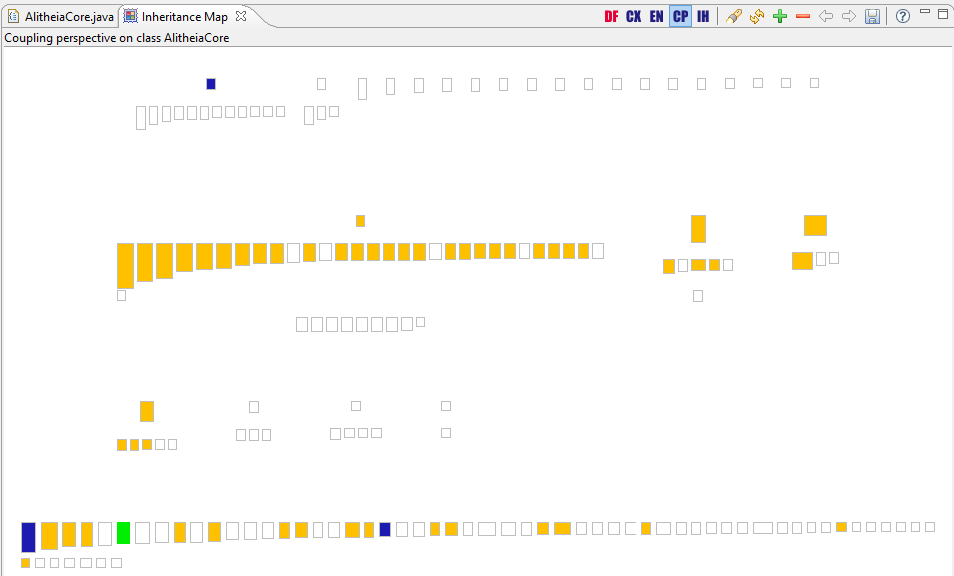
\includegraphics[width=0.8\textwidth]{alitheiacore-coupling}
    \caption{AlitheiaCore coupling}
    \label{fig:alitheiacore}
\end{figure}

From the inheritance map we observe that \verb|DAObject| (figure~\ref{fig:daobject}) and \verb|AlitheiaCoreService| (figure~\ref{fig:alitheacoreservice}) have a lot of subclasses.	The subclasses of \verb|AlitheiaCoreService| are interfaces for each service.

\begin{figure}[h]
\centering
\begin{minipage}{.5\textwidth}
  \centering
  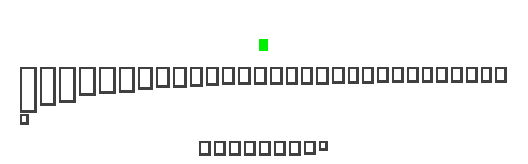
\includegraphics[width=0.9\linewidth]{daoobject-inheritance}
  \captionof{figure}{DAObject (green) with subclasses (bordered)}
  \label{fig:daobject}
\end{minipage}%
\begin{minipage}{.5\textwidth}
  \centering
  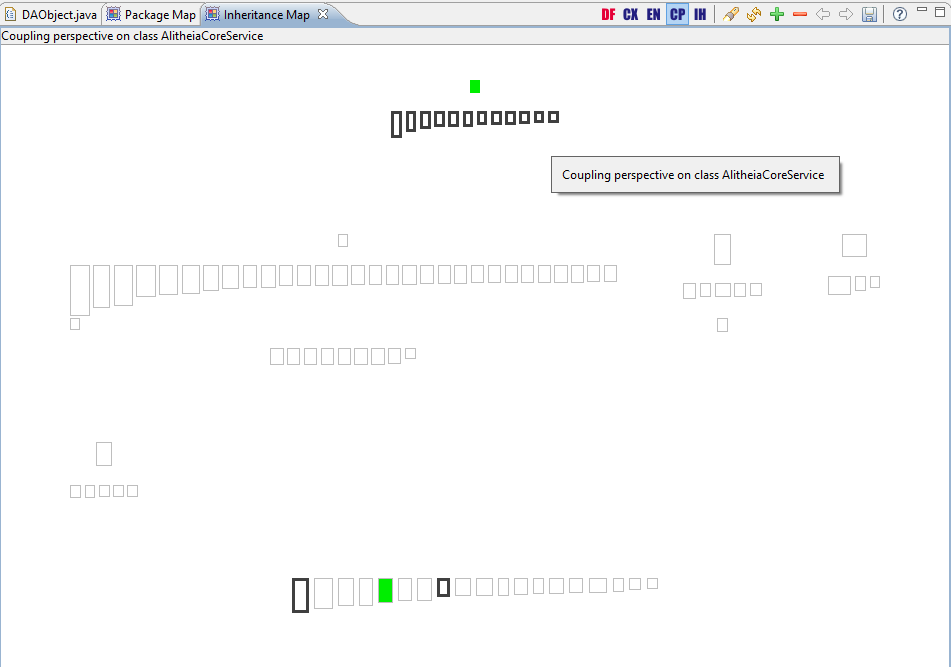
\includegraphics[width=0.9\linewidth]{alitheiacoreservice-inheritance}
  \captionof{figure}{AlitheiaCoreService (green) with subclasses (bordered)}
  \label{fig:alitheacoreservice}
\end{minipage}
\end{figure}

\section{Problem Detection}

\subsection{SRP violation}
\label{sec:srp}
\begin{enumerate}
\item The abstract class \verb|Job| contains a lot of methods. Its main responsibility is to represent the concept of a `job'. To accomplish this it contains properties (e.g. state, dependencies, dependees) and methods (addDependency, removeDependency, dependsOn) to alter its state. However, the class also exposes a method called verb|execute()|. This indicates that the \verb|Job| class is also responsible for executing a job. We argue that this is a violation of the SRP, because there is more than one motive for chaning the \verb|Job| class: either if the way we represent a job changes, or if the way we execute a job changes. A better architecture would be to move the job execution out of the \verb|Job| class and into a service layer (for example, \verb|JobExecuter|).

% Refs: www.objectmentor.com/resources/articles/srp.pdf, https://twitter.com/jeffrey_way/status/527857091470700544, http://verraes.net/2014/09/objects-as-contracts-for-behaviour/, http://msdn.microsoft.com/en-gb/magazine/dn385704.aspx, https://blog.inf.ed.ac.uk/sapm/2014/02/04/the-anaemic-domain-model-is-no-anti-pattern-its-a-solid-design/

\item The class \verb|ProjectsView.java|: its name suggests that it renders HTML output, but it also takes care of parsing the servlet's request object, adding projects, removing projects, and triggering updates.

\item Model classes should represent the corresponding domain entity, the whole domain entity and nothing but the domain entity. The class \verb|Bug| should represent a bug. It should not be aware of the way in which it is persisted (it should not be awere whether it is persisted at all). The current implementation of \verb|Bug.java| contains SQL queries for retrieving the information from the database and constructing the object, which is a major violation of the SRP principle.

% \item The ProjectEvent interface delcares a getEventPriority method and RepositoryEvent, MailingListEvent, and BugDBEvent implement this method. However, each class returns a constant. This indicates that event priority is actually not a property of these events. Diving a bit deeper we see that this method is used to compare ProjectEvent's. A correct way to implement this would be to create a custom comparator, which inspects the runtime type to compare two ProjectEvents. This is more extensible then returning integers (imaging creating an event that has property between two existing properties) and more maintainable.
\end{enumerate}

\subsection{OCP/LSP violation}
The \verb|Metric| class contains a property \verb|metricType: MetricType|. The \verb|MetricType| contains a \verb|Type| enumeration of types and a property \verb|type: String|. This indicates an overcomplicated design, because the \verb|MetricType| class does not add anything to the \verb|Type| enumeration (except the data access method \verb|getMetricType| that should not be there in the first place, see section~\ref{sec:srp}).

The \verb|Metric.java| class contains a method \verb|isEvaluated(StoredProject)|. This method contains a switch statements on a metric's type's enum type. Depending on the metric type's enum type, a different query is constructed. This is not open for modification, because we need to change the \verb|Metric| class if a new type is added in the future. To solve this issue, we suggest adding a \verb|isEvaluated(): String| method to a \verb|MetricType| interface from which all \verb|MetricType|'s must inherit. The \verb|isEvaluated(StoredProject)| method can then rely on the \verb|MetricType| interface.

We found this issue by searching for usages of `switch' in IntelliJ.

\subsection{DIP violation}
The class \verb|CacheServiceImpl| instantiates a subclass of itself. Being aware of your subclasses violates the DIP. The class should depend on abstractions instead of implementations.

The interface \verb|eu.sqooss.service.fds.InMemoryCheckout| depends on the low level \verb|eu.sqooss.service.fds.InMemoryDirectory| which is a violation of the Dependency Inversion Principle. % TODO: Uitbereiden, dit komt "overal" voor

\subsection{ADP violation}
% definitie ADP uitleggen
% alle cycles met AlitheiaCore.java

\subsection{DRY violation}
In the class eu.sqooss.service.db.ProjectVersion a lot of duplicate is shared between the getLiveFilesCount and getVersionFiles methods. 

Furthermore, in the same class the methods getVersionByRevision and getVersionByTimestamp are exactly the same aside from one parameter.

% per principle:
% - wat het inhoud
% - hoe we gezocht hebben
% - wat we gevonden hebben

\subsection{Further examples}
Further examples of violations of class and package design (optionally!)
 - The system uses AlitheiaCore for providing implementations for certain interfaces, which is better than relying on implementations. However, this can be taken one step further by applying IoC: instead of creating your dependencies, you declare your dependencies and let someone higher up take care of creating them. This increases decoupling and makes maintaining code easier.
 - Dead code. See \verb|DiskUtil.java| createTestFiles, and the \verb|static final int|'s you find above and below in that file. Also, \verb|Parser.java| is not used.
 - Comments containing TODO or FIXME. Though this is not necessarily harmful, it would be better to store these in an issue tracker. That also allows for a more meaningful description than ``this can break''.
 - Commented code. For example, \verb|Developer.java| contains two places with commented code. We suggest using a version control system and only storing production-ready code in the master branch.

\bibliographystyle{plain}
\bibliography{report}

\end{document}